\documentclass[]{book}
\usepackage{lmodern}
\usepackage{amssymb,amsmath}
\usepackage{ifxetex,ifluatex}
\usepackage{fixltx2e} % provides \textsubscript
\ifnum 0\ifxetex 1\fi\ifluatex 1\fi=0 % if pdftex
  \usepackage[T1]{fontenc}
  \usepackage[utf8]{inputenc}
\else % if luatex or xelatex
  \ifxetex
    \usepackage{mathspec}
  \else
    \usepackage{fontspec}
  \fi
  \defaultfontfeatures{Ligatures=TeX,Scale=MatchLowercase}
\fi
% use upquote if available, for straight quotes in verbatim environments
\IfFileExists{upquote.sty}{\usepackage{upquote}}{}
% use microtype if available
\IfFileExists{microtype.sty}{%
\usepackage{microtype}
\UseMicrotypeSet[protrusion]{basicmath} % disable protrusion for tt fonts
}{}
\usepackage[margin=1in]{geometry}
\usepackage{hyperref}
\hypersetup{unicode=true,
            pdftitle={Applied SNA with R},
            pdfauthor={George G. Vega Yon},
            pdfborder={0 0 0},
            breaklinks=true}
\urlstyle{same}  % don't use monospace font for urls
\usepackage{natbib}
\bibliographystyle{apalike}
\usepackage{color}
\usepackage{fancyvrb}
\newcommand{\VerbBar}{|}
\newcommand{\VERB}{\Verb[commandchars=\\\{\}]}
\DefineVerbatimEnvironment{Highlighting}{Verbatim}{commandchars=\\\{\}}
% Add ',fontsize=\small' for more characters per line
\usepackage{framed}
\definecolor{shadecolor}{RGB}{248,248,248}
\newenvironment{Shaded}{\begin{snugshade}}{\end{snugshade}}
\newcommand{\KeywordTok}[1]{\textcolor[rgb]{0.13,0.29,0.53}{\textbf{#1}}}
\newcommand{\DataTypeTok}[1]{\textcolor[rgb]{0.13,0.29,0.53}{#1}}
\newcommand{\DecValTok}[1]{\textcolor[rgb]{0.00,0.00,0.81}{#1}}
\newcommand{\BaseNTok}[1]{\textcolor[rgb]{0.00,0.00,0.81}{#1}}
\newcommand{\FloatTok}[1]{\textcolor[rgb]{0.00,0.00,0.81}{#1}}
\newcommand{\ConstantTok}[1]{\textcolor[rgb]{0.00,0.00,0.00}{#1}}
\newcommand{\CharTok}[1]{\textcolor[rgb]{0.31,0.60,0.02}{#1}}
\newcommand{\SpecialCharTok}[1]{\textcolor[rgb]{0.00,0.00,0.00}{#1}}
\newcommand{\StringTok}[1]{\textcolor[rgb]{0.31,0.60,0.02}{#1}}
\newcommand{\VerbatimStringTok}[1]{\textcolor[rgb]{0.31,0.60,0.02}{#1}}
\newcommand{\SpecialStringTok}[1]{\textcolor[rgb]{0.31,0.60,0.02}{#1}}
\newcommand{\ImportTok}[1]{#1}
\newcommand{\CommentTok}[1]{\textcolor[rgb]{0.56,0.35,0.01}{\textit{#1}}}
\newcommand{\DocumentationTok}[1]{\textcolor[rgb]{0.56,0.35,0.01}{\textbf{\textit{#1}}}}
\newcommand{\AnnotationTok}[1]{\textcolor[rgb]{0.56,0.35,0.01}{\textbf{\textit{#1}}}}
\newcommand{\CommentVarTok}[1]{\textcolor[rgb]{0.56,0.35,0.01}{\textbf{\textit{#1}}}}
\newcommand{\OtherTok}[1]{\textcolor[rgb]{0.56,0.35,0.01}{#1}}
\newcommand{\FunctionTok}[1]{\textcolor[rgb]{0.00,0.00,0.00}{#1}}
\newcommand{\VariableTok}[1]{\textcolor[rgb]{0.00,0.00,0.00}{#1}}
\newcommand{\ControlFlowTok}[1]{\textcolor[rgb]{0.13,0.29,0.53}{\textbf{#1}}}
\newcommand{\OperatorTok}[1]{\textcolor[rgb]{0.81,0.36,0.00}{\textbf{#1}}}
\newcommand{\BuiltInTok}[1]{#1}
\newcommand{\ExtensionTok}[1]{#1}
\newcommand{\PreprocessorTok}[1]{\textcolor[rgb]{0.56,0.35,0.01}{\textit{#1}}}
\newcommand{\AttributeTok}[1]{\textcolor[rgb]{0.77,0.63,0.00}{#1}}
\newcommand{\RegionMarkerTok}[1]{#1}
\newcommand{\InformationTok}[1]{\textcolor[rgb]{0.56,0.35,0.01}{\textbf{\textit{#1}}}}
\newcommand{\WarningTok}[1]{\textcolor[rgb]{0.56,0.35,0.01}{\textbf{\textit{#1}}}}
\newcommand{\AlertTok}[1]{\textcolor[rgb]{0.94,0.16,0.16}{#1}}
\newcommand{\ErrorTok}[1]{\textcolor[rgb]{0.64,0.00,0.00}{\textbf{#1}}}
\newcommand{\NormalTok}[1]{#1}
\usepackage{longtable,booktabs}
\usepackage{graphicx,grffile}
\makeatletter
\def\maxwidth{\ifdim\Gin@nat@width>\linewidth\linewidth\else\Gin@nat@width\fi}
\def\maxheight{\ifdim\Gin@nat@height>\textheight\textheight\else\Gin@nat@height\fi}
\makeatother
% Scale images if necessary, so that they will not overflow the page
% margins by default, and it is still possible to overwrite the defaults
% using explicit options in \includegraphics[width, height, ...]{}
\setkeys{Gin}{width=\maxwidth,height=\maxheight,keepaspectratio}
\IfFileExists{parskip.sty}{%
\usepackage{parskip}
}{% else
\setlength{\parindent}{0pt}
\setlength{\parskip}{6pt plus 2pt minus 1pt}
}
\setlength{\emergencystretch}{3em}  % prevent overfull lines
\providecommand{\tightlist}{%
  \setlength{\itemsep}{0pt}\setlength{\parskip}{0pt}}
\setcounter{secnumdepth}{5}
% Redefines (sub)paragraphs to behave more like sections
\ifx\paragraph\undefined\else
\let\oldparagraph\paragraph
\renewcommand{\paragraph}[1]{\oldparagraph{#1}\mbox{}}
\fi
\ifx\subparagraph\undefined\else
\let\oldsubparagraph\subparagraph
\renewcommand{\subparagraph}[1]{\oldsubparagraph{#1}\mbox{}}
\fi

%%% Use protect on footnotes to avoid problems with footnotes in titles
\let\rmarkdownfootnote\footnote%
\def\footnote{\protect\rmarkdownfootnote}

%%% Change title format to be more compact
\usepackage{titling}

% Create subtitle command for use in maketitle
\newcommand{\subtitle}[1]{
  \posttitle{
    \begin{center}\large#1\end{center}
    }
}

\setlength{\droptitle}{-2em}
  \title{Applied SNA with R}
  \pretitle{\vspace{\droptitle}\centering\huge}
  \posttitle{\par}
  \author{George G. Vega Yon}
  \preauthor{\centering\large\emph}
  \postauthor{\par}
  \predate{\centering\large\emph}
  \postdate{\par}
  \date{2018-02-02}

\usepackage{booktabs}
\usepackage{hyperref}
  \hypersetup{allcolors=blue, colorlinks=true}

\usepackage{amsthm}
\newtheorem{theorem}{Theorem}[chapter]
\newtheorem{lemma}{Lemma}[chapter]
\theoremstyle{definition}
\newtheorem{definition}{Definition}[chapter]
\newtheorem{corollary}{Corollary}[chapter]
\newtheorem{proposition}{Proposition}[chapter]
\theoremstyle{definition}
\newtheorem{example}{Example}[chapter]
\theoremstyle{definition}
\newtheorem{exercise}{Exercise}[chapter]
\theoremstyle{remark}
\newtheorem*{remark}{Remark}
\newtheorem*{solution}{Solution}
\begin{document}
\maketitle

{
\setcounter{tocdepth}{1}
\tableofcontents
}
\chapter{About this book}\label{about-this-book}

This book will be build as part of a workshop on Applied Social Network
Analysis with R. Its contents will be populated as the sessions take
place, and for now there is particular program that we will follow,
instead, we have the following workflow:

\begin{enumerate}
\def\labelenumi{\arabic{enumi}.}
\item
  Participants will share their data and what they need to do with it.
\item
  Based on their data, I'll be preparing the sessions trying to show
  attendees how would I approach the problem, and at the same time,
  teach by example about the R language.
\item
  Materials will be published on this website and, hopefully, video
  recordings of the sessions.
\end{enumerate}

At least in the first version, the book will be organized by session,
this is, one chapter per session.

All the book materials can be downloaded from
\url{https://github.com/gvegayon/appliedsnar}

In general, we will besides of R itself, we will be using R studio and
the following R packages: dplyr for data management, stringr for data
cleaning, and of course igraph, netdiffuseR (a bit of a bias here), and
statnet for our neat network analysis.\footnote{Some of you may be
  wondering ``what about ggplot2 and friends? What about
  \href{https://www.tidyverse.org/}{\texttt{tidyverse}}'', well, my
  short answer is I jumped into R before all of that was that popular.
  When I started plots were all about
  \href{https://CRAN.R-project.org/package=lattice}{\texttt{lattice}},
  and after a couple of years on that, about base R graphics. What I'm
  saying is that so far I have not find a compelling reason to leave my
  ``old-practices'' and embrace all the \texttt{tidyverse} movement
  (religion?).}

\chapter{Introduction}\label{introduction}

For this book we need the following

\begin{enumerate}
\def\labelenumi{\arabic{enumi}.}
\item
  Install R from CRAN: \url{https://www.r-project.org/}
\item
  (optional) Install Rstudio: \url{https://rstudio.org}
\end{enumerate}

While I find RStudio extreamly useful, it is not necesary to use it with
R.

\chapter{R Basics}\label{r-basics}

\section{What is R}\label{what-is-r}

\section{How to install packages}\label{how-to-install-packages}

Nowadays there are two ways of installing R packages (that I'm aware
of), either using \texttt{install.packages}, which is a function shipped
with R, or use the devtools R package to install a package from some
remote repository other than CRAN, here is a couple of examples:

\begin{Shaded}
\begin{Highlighting}[]
\CommentTok{# This will install the igraph package from CRAN}
\OperatorTok{>}\StringTok{ }\KeywordTok{install.packages}\NormalTok{(}\StringTok{"netdiffuseR"}\NormalTok{)}

\CommentTok{# This will install the bleeding-edge version from the project's github repo!}
\OperatorTok{>}\StringTok{ }\NormalTok{devtools}\OperatorTok{::}\KeywordTok{install_github}\NormalTok{(}\StringTok{"USCCANA/netdiffuseR"}\NormalTok{)}
\end{Highlighting}
\end{Shaded}

The first one, using \texttt{install.packages}, installs the CRAN
version of \texttt{netdiffuseR}, whereas the second installs whatever
version is plublished on \url{https://github.com/USCCANA/netdiffuseR},
which is usually called the development version.

In some cases users may want/need to install packages from command line
as some packages need extra configuration to be installed. But we won't
need to look at it now.

\chapter{Week 1: SNS Study}\label{week-1-sns-study}

The data can be downloaded from
\href{https://cdn.rawgit.com/gvegayon/appliedsnar/fdc0d26f/03-sns.dta}{here}.

The codebook for the data provided here is in
\protect\hyperlink{sns-data}{the appendix}.

This chapter's goals are:

\begin{enumerate}
\def\labelenumi{\arabic{enumi}.}
\item
  Read the data into R,
\item
  Create a network with it,
\item
  Compute descriptive statistics
\item
  Visualize the network
\end{enumerate}

\section{Data preprocessing}\label{data-preprocessing}

\subsection{Reading the data into R}\label{reading-the-data-into-r}

R has several ways of reading data in. You data can be Raw plain files
like CSV, tab delimited or specified by column width, for which you can
use the \href{https://cran.r-project.org/package=readr}{\texttt{readr}}
package; or it can be binary files like dta (Stata), Octave, SPSS, for
which \href{https://cran.r-project.org/package=readr}{\texttt{foreign}}
can be used; or it could be excel files in which case you should be
using \href{https://cran.r-project.org/package=readxl}{\texttt{readxl}}.
In our case, the data for this session is in Stata format:

\begin{Shaded}
\begin{Highlighting}[]
\KeywordTok{library}\NormalTok{(dplyr)}
\KeywordTok{library}\NormalTok{(magrittr)}
\KeywordTok{library}\NormalTok{(foreign)}

\CommentTok{# Reading the data}
\NormalTok{dat <-}\StringTok{ }\NormalTok{foreign}\OperatorTok{::}\KeywordTok{read.dta}\NormalTok{(}\StringTok{"03-sns.dta"}\NormalTok{)}

\CommentTok{# Taking a look at the data's first 5 columns and 5 rows}
\NormalTok{dat[}\DecValTok{1}\OperatorTok{:}\DecValTok{5}\NormalTok{, }\DecValTok{1}\OperatorTok{:}\DecValTok{10}\NormalTok{]}
\end{Highlighting}
\end{Shaded}

\begin{verbatim}
##   photoid school hispanic female1 female2 female3 female4 grades1 grades2
## 1       1    111        1      NA      NA       0       0      NA      NA
## 2       2    111        1       0      NA      NA       0     3.0      NA
## 3       7    111        0       1       1       1       1     5.0     4.5
## 4      13    111        1       1       1       1       1     2.5     2.5
## 5      14    111        1       1       1       1      NA     3.0     3.5
##   grades3
## 1     3.5
## 2      NA
## 3     4.0
## 4     2.5
## 5     3.5
\end{verbatim}

\subsection{Creating a unique id for each
participant}\label{creating-a-unique-id-for-each-participant}

Now suppose that we want to create a unique id using the school and
photo id. In this case, since both variables are numeric, a good way of
doing it is to encode the id such that, for example, the last three
\texttt{x} numbers are the photoid and the first ones are the school id.
To do this we need to take into account the range of the variables.
Here, \texttt{photoid} has the following range:

\begin{Shaded}
\begin{Highlighting}[]
\NormalTok{(photo_id_ran <-}\StringTok{ }\KeywordTok{range}\NormalTok{(dat}\OperatorTok{$}\NormalTok{photoid))}
\end{Highlighting}
\end{Shaded}

\begin{verbatim}
## [1]    1 2074
\end{verbatim}

As the variable spans up to 2074, we need to set the last 4 units of the
variable to store the \texttt{photoid}. Again, we use \texttt{dplyr} to
create this variable, and we will call it\ldots{} \texttt{id} (mind
blowing, right?):

\begin{Shaded}
\begin{Highlighting}[]
\NormalTok{(dat }\OperatorTok\StringTok{ }\KeywordTok{mutate}\NormalTok{(}\DataTypeTok{id =}\NormalTok{ school}\OperatorTok{*}\DecValTok{10000} \OperatorTok{+}\StringTok{ }\NormalTok{photoid)) }\OperatorTok
\StringTok{  }\NormalTok{head }\OperatorTok
\StringTok{  }\KeywordTok{select}\NormalTok{(school, photoid, id)}
\end{Highlighting}
\end{Shaded}

\begin{verbatim}
##   school photoid      id
## 1    111       1 1110001
## 2    111       2 1110002
## 3    111       7 1110007
## 4    111      13 1110013
## 5    111      14 1110014
## 6    111      15 1110015
\end{verbatim}

Wow, what happend in the last three lines of code! What is that
\texttt{\%\textgreater{}\%}? Well, that's the
\href{http://r4ds.had.co.nz/pipes.html}{piping operator}, and it is a
very nice way of writing nested function calls. In this case, instead of
having write something like

\begin{Shaded}
\begin{Highlighting}[]
\NormalTok{dat_filtered}\OperatorTok{$}\NormalTok{id <-}\StringTok{ }\NormalTok{dat_filtered}\OperatorTok{$}\NormalTok{school}\OperatorTok{*}\DecValTok{10000} \OperatorTok{+}\StringTok{ }\NormalTok{dat_filtered}\OperatorTok{$}\NormalTok{photoid}
\KeywordTok{subset}\NormalTok{(}\KeywordTok{head}\NormalTok{(dat_filtered), }\DataTypeTok{select =} \KeywordTok{c}\NormalTok{(school, photoid, id))}
\end{Highlighting}
\end{Shaded}

\section{Creating a network}\label{creating-a-network}

\begin{itemize}
\item
  We want to build a social network. For that, we either use an
  adjacency matrix or an edgelist.
\item
  Each individual of the SNS data nomitated 19 friends from school. We
  will use those nominations to create the social network.
\item
  In this case, we will create the network by coercing the dataset into
  an edgelist.
\end{itemize}

\subsection{From survey to edgelist}\label{from-survey-to-edgelist}

Let's start by loading a couple of handy R packages for this task.

\begin{Shaded}
\begin{Highlighting}[]
\KeywordTok{library}\NormalTok{(tidyr)}
\KeywordTok{library}\NormalTok{(stringr)}
\end{Highlighting}
\end{Shaded}

Optionally, we can use the \texttt{tibble} type of object which is an
alternative to the actual \texttt{data.frame}. This object is claimed to
provide \emph{more efficient methods for matrices and data frames}.

\begin{Shaded}
\begin{Highlighting}[]
\NormalTok{dat <-}\StringTok{ }\KeywordTok{as_tibble}\NormalTok{(dat)}
\end{Highlighting}
\end{Shaded}

What I like from tibbles is that when you print them on the console
these actually look nice:

\begin{Shaded}
\begin{Highlighting}[]
\NormalTok{dat}
\end{Highlighting}
\end{Shaded}

\begin{verbatim}
## # A tibble: 2,164 x 100
##    photoid school hispanic female1 female2 female3 female4 grades1 grades2
##      <int>  <int>    <dbl>   <int>   <int>   <int>   <int>   <dbl>   <dbl>
##  1       1    111     1.00      NA      NA       0       0   NA      NA   
##  2       2    111     1.00       0      NA      NA       0    3.00   NA   
##  3       7    111     0          1       1       1       1    5.00    4.50
##  4      13    111     1.00       1       1       1       1    2.50    2.50
##  5      14    111     1.00       1       1       1      NA    3.00    3.50
##  6      15    111     1.00       0       0       0       0    2.50    2.50
##  7      20    111     1.00       1       1       1       1    2.50    2.50
##  8      22    111     1.00      NA      NA       0       0   NA      NA   
##  9      25    111     0          1       1      NA       1    4.50    3.50
## 10      27    111     1.00       0      NA       0       0    3.50   NA   
## # ... with 2,154 more rows, and 91 more variables: grades3 <dbl>,
## #   grades4 <dbl>, eversmk1 <int>, eversmk2 <int>, eversmk3 <int>,
## #   eversmk4 <int>, everdrk1 <int>, everdrk2 <int>, everdrk3 <int>,
## #   everdrk4 <int>, home1 <int>, home2 <int>, home3 <int>, home4 <int>,
## #   sch_friend11 <int>, sch_friend12 <int>, sch_friend13 <int>,
## #   sch_friend14 <int>, sch_friend15 <int>, sch_friend16 <int>,
## #   sch_friend17 <int>, sch_friend18 <int>, sch_friend19 <int>,
## #   sch_friend110 <int>, sch_friend111 <int>, sch_friend112 <int>,
## #   sch_friend113 <int>, sch_friend114 <int>, sch_friend115 <int>,
## #   sch_friend116 <int>, sch_friend117 <int>, sch_friend118 <int>,
## #   sch_friend119 <int>, sch_friend21 <int>, sch_friend22 <int>,
## #   sch_friend23 <int>, sch_friend24 <int>, sch_friend25 <int>,
## #   sch_friend26 <int>, sch_friend27 <int>, sch_friend28 <int>,
## #   sch_friend29 <int>, sch_friend210 <int>, sch_friend211 <int>,
## #   sch_friend212 <int>, sch_friend213 <int>, sch_friend214 <int>,
## #   sch_friend215 <int>, sch_friend216 <int>, sch_friend217 <int>,
## #   sch_friend218 <int>, sch_friend219 <int>, sch_friend31 <int>,
## #   sch_friend32 <int>, sch_friend33 <int>, sch_friend34 <int>,
## #   sch_friend35 <int>, sch_friend36 <int>, sch_friend37 <int>,
## #   sch_friend38 <int>, sch_friend39 <int>, sch_friend310 <int>,
## #   sch_friend311 <int>, sch_friend312 <int>, sch_friend313 <int>,
## #   sch_friend314 <int>, sch_friend315 <int>, sch_friend316 <int>,
## #   sch_friend317 <int>, sch_friend318 <int>, sch_friend319 <int>,
## #   sch_friend41 <int>, sch_friend42 <int>, sch_friend43 <int>,
## #   sch_friend44 <int>, sch_friend45 <int>, sch_friend46 <int>,
## #   sch_friend47 <int>, sch_friend48 <int>, sch_friend49 <int>,
## #   sch_friend410 <int>, sch_friend411 <int>, sch_friend412 <int>,
## #   sch_friend413 <int>, sch_friend414 <int>, sch_friend415 <int>,
## #   sch_friend416 <int>, sch_friend417 <int>, sch_friend418 <int>,
## #   sch_friend419 <int>, id <dbl>
\end{verbatim}

\begin{Shaded}
\begin{Highlighting}[]
\CommentTok{# Maybe too much piping... but its cool!}
\NormalTok{net <-}\StringTok{ }\NormalTok{dat }\OperatorTok\StringTok{ }
\StringTok{  }\KeywordTok{select}\NormalTok{(id, school, }\KeywordTok{starts_with}\NormalTok{(}\StringTok{"sch_friend"}\NormalTok{)) }\OperatorTok
\StringTok{  }\KeywordTok{gather}\NormalTok{(}\DataTypeTok{key =} \StringTok{"varname"}\NormalTok{, }\DataTypeTok{value =} \StringTok{"content"}\NormalTok{, }\OperatorTok{-}\NormalTok{id, }\OperatorTok{-}\NormalTok{school) }\OperatorTok
\StringTok{  }\KeywordTok{filter}\NormalTok{(}\OperatorTok{!}\KeywordTok{is.na}\NormalTok{(content)) }\OperatorTok
\StringTok{  }\KeywordTok{mutate}\NormalTok{(}
    \DataTypeTok{friendid =}\NormalTok{ school}\OperatorTok{*}\DecValTok{10000} \OperatorTok{+}\StringTok{ }\NormalTok{content,}
    \DataTypeTok{year     =} \KeywordTok{str_extract}\NormalTok{(varname, }\StringTok{"(?<=[a-z])[0-9]"}\NormalTok{),}
    \DataTypeTok{nnom     =} \KeywordTok{str_extract}\NormalTok{(varname, }\StringTok{"(?<=[a-z][0-9])[0-9]+"}\NormalTok{)}
\NormalTok{  )}
\end{Highlighting}
\end{Shaded}

Let's take a look at this step by step:

\begin{enumerate}
\def\labelenumi{\arabic{enumi}.}
\item
  First, we subset the data: We want to keep
  \texttt{id,\ school,\ sch\_friend*}. For the later we use the function
  \texttt{starts\_with} (from the \texttt{tidyselect} package). This
  allows us to select all variables that starts with the word
  ``\texttt{sch\_friend}'', which means that
  \texttt{sch\_friend11,\ sch\_friend12,\ ...} will all be selected.

\begin{Shaded}
\begin{Highlighting}[]
\NormalTok{dat }\OperatorTok\StringTok{ }
\StringTok{  }\KeywordTok{select}\NormalTok{(id, school, }\KeywordTok{starts_with}\NormalTok{(}\StringTok{"sch_friend"}\NormalTok{))}
\end{Highlighting}
\end{Shaded}

\begin{verbatim}
## # A tibble: 2,164 x 78
##         id school sch_friend11 sch_friend12 sch_friend13 sch_friend14
##      <dbl>  <int>        <int>        <int>        <int>        <int>
##  1 1110001    111           NA           NA           NA           NA
##  2 1110002    111          424          423          426          289
##  3 1110007    111          629          505           NA           NA
##  4 1110013    111          232          569           NA           NA
##  5 1110014    111          582          134           41          592
##  6 1110015    111           26          488           81          138
##  7 1110020    111          528           NA          492          395
##  8 1110022    111           NA           NA           NA           NA
##  9 1110025    111          135          185          553           84
## 10 1110027    111          346          168          559            5
## # ... with 2,154 more rows, and 72 more variables: sch_friend15 <int>,
## #   sch_friend16 <int>, sch_friend17 <int>, sch_friend18 <int>,
## #   sch_friend19 <int>, sch_friend110 <int>, sch_friend111 <int>,
## #   sch_friend112 <int>, sch_friend113 <int>, sch_friend114 <int>,
## #   sch_friend115 <int>, sch_friend116 <int>, sch_friend117 <int>,
## #   sch_friend118 <int>, sch_friend119 <int>, sch_friend21 <int>,
## #   sch_friend22 <int>, sch_friend23 <int>, sch_friend24 <int>,
## #   sch_friend25 <int>, sch_friend26 <int>, sch_friend27 <int>,
## #   sch_friend28 <int>, sch_friend29 <int>, sch_friend210 <int>,
## #   sch_friend211 <int>, sch_friend212 <int>, sch_friend213 <int>,
## #   sch_friend214 <int>, sch_friend215 <int>, sch_friend216 <int>,
## #   sch_friend217 <int>, sch_friend218 <int>, sch_friend219 <int>,
## #   sch_friend31 <int>, sch_friend32 <int>, sch_friend33 <int>,
## #   sch_friend34 <int>, sch_friend35 <int>, sch_friend36 <int>,
## #   sch_friend37 <int>, sch_friend38 <int>, sch_friend39 <int>,
## #   sch_friend310 <int>, sch_friend311 <int>, sch_friend312 <int>,
## #   sch_friend313 <int>, sch_friend314 <int>, sch_friend315 <int>,
## #   sch_friend316 <int>, sch_friend317 <int>, sch_friend318 <int>,
## #   sch_friend319 <int>, sch_friend41 <int>, sch_friend42 <int>,
## #   sch_friend43 <int>, sch_friend44 <int>, sch_friend45 <int>,
## #   sch_friend46 <int>, sch_friend47 <int>, sch_friend48 <int>,
## #   sch_friend49 <int>, sch_friend410 <int>, sch_friend411 <int>,
## #   sch_friend412 <int>, sch_friend413 <int>, sch_friend414 <int>,
## #   sch_friend415 <int>, sch_friend416 <int>, sch_friend417 <int>,
## #   sch_friend418 <int>, sch_friend419 <int>
\end{verbatim}
\item
  Then, we reshape it to \emph{long} format: By transposing all the
  \texttt{sch\_friend*} to long. We do this by means of the function
  \texttt{gather} (from the \texttt{tidyr} package). This is an
  alternative to the \texttt{reshape} function, and I personally find it
  easier to use. Let's see how it works:

\begin{Shaded}
\begin{Highlighting}[]
\NormalTok{dat }\OperatorTok\StringTok{ }
\StringTok{  }\KeywordTok{select}\NormalTok{(id, school, }\KeywordTok{starts_with}\NormalTok{(}\StringTok{"sch_friend"}\NormalTok{)) }\OperatorTok
\StringTok{  }\KeywordTok{gather}\NormalTok{(}\DataTypeTok{key =} \StringTok{"varname"}\NormalTok{, }\DataTypeTok{value =} \StringTok{"content"}\NormalTok{, }\OperatorTok{-}\NormalTok{id, }\OperatorTok{-}\NormalTok{school)}
\end{Highlighting}
\end{Shaded}

\begin{verbatim}
## # A tibble: 164,464 x 4
##         id school varname      content
##      <dbl>  <int> <chr>          <int>
##  1 1110001    111 sch_friend11      NA
##  2 1110002    111 sch_friend11     424
##  3 1110007    111 sch_friend11     629
##  4 1110013    111 sch_friend11     232
##  5 1110014    111 sch_friend11     582
##  6 1110015    111 sch_friend11      26
##  7 1110020    111 sch_friend11     528
##  8 1110022    111 sch_friend11      NA
##  9 1110025    111 sch_friend11     135
## 10 1110027    111 sch_friend11     346
## # ... with 164,454 more rows
\end{verbatim}

  In this case the \texttt{key} parameter sets the name of the variable
  that will contain the name of the variable that was reshaped, while
  \texttt{value} is the name of the variable that will hold the content
  of the data (that's why I named those like that). The
  \texttt{-id,\ -school} bit tells the function to ``drop'' those
  variables before reshaping, in other words, ``reshape everything but
  \texttt{id} and \texttt{school}''.

  Also, notice that we passed from 2164 rows to 19 (nominations) * 2164
  (subjects) * 4 (waves) = 164464 rows, as expected.
\item
  As the nomination data can be empty for some cells, we need to take
  care of those cases, the \texttt{NA}s, so we filter the data:

\begin{Shaded}
\begin{Highlighting}[]
\NormalTok{dat }\OperatorTok\StringTok{ }
\StringTok{  }\KeywordTok{select}\NormalTok{(id, school, }\KeywordTok{starts_with}\NormalTok{(}\StringTok{"sch_friend"}\NormalTok{)) }\OperatorTok
\StringTok{  }\KeywordTok{gather}\NormalTok{(}\DataTypeTok{key =} \StringTok{"varname"}\NormalTok{, }\DataTypeTok{value =} \StringTok{"content"}\NormalTok{, }\OperatorTok{-}\NormalTok{id, }\OperatorTok{-}\NormalTok{school) }\OperatorTok
\StringTok{  }\KeywordTok{filter}\NormalTok{(}\OperatorTok{!}\KeywordTok{is.na}\NormalTok{(content))}
\end{Highlighting}
\end{Shaded}

\begin{verbatim}
## # A tibble: 39,561 x 4
##         id school varname      content
##      <dbl>  <int> <chr>          <int>
##  1 1110002    111 sch_friend11     424
##  2 1110007    111 sch_friend11     629
##  3 1110013    111 sch_friend11     232
##  4 1110014    111 sch_friend11     582
##  5 1110015    111 sch_friend11      26
##  6 1110020    111 sch_friend11     528
##  7 1110025    111 sch_friend11     135
##  8 1110027    111 sch_friend11     346
##  9 1110029    111 sch_friend11     369
## 10 1110030    111 sch_friend11     462
## # ... with 39,551 more rows
\end{verbatim}
\item
  And finally, we create three new variables from this dataset:
  \texttt{friendid}, \texttt{year}, and \texttt{nom\_num} (nomination
  number). All this using regular expressions:

\begin{Shaded}
\begin{Highlighting}[]
\NormalTok{dat }\OperatorTok\StringTok{ }
\StringTok{  }\KeywordTok{select}\NormalTok{(id, school, }\KeywordTok{starts_with}\NormalTok{(}\StringTok{"sch_friend"}\NormalTok{)) }\OperatorTok
\StringTok{  }\KeywordTok{gather}\NormalTok{(}\DataTypeTok{key =} \StringTok{"varname"}\NormalTok{, }\DataTypeTok{value =} \StringTok{"content"}\NormalTok{, }\OperatorTok{-}\NormalTok{id, }\OperatorTok{-}\NormalTok{school) }\OperatorTok
\StringTok{  }\KeywordTok{filter}\NormalTok{(}\OperatorTok{!}\KeywordTok{is.na}\NormalTok{(content)) }\OperatorTok
\StringTok{  }\KeywordTok{mutate}\NormalTok{(}
    \DataTypeTok{friendid =}\NormalTok{ school}\OperatorTok{*}\DecValTok{10000} \OperatorTok{+}\StringTok{ }\NormalTok{content,}
    \DataTypeTok{year     =} \KeywordTok{str_extract}\NormalTok{(varname, }\StringTok{"(?<=[a-z])[0-9]"}\NormalTok{),}
    \DataTypeTok{nnom     =} \KeywordTok{str_extract}\NormalTok{(varname, }\StringTok{"(?<=[a-z][0-9])[0-9]+"}\NormalTok{)}
\NormalTok{    )}
\end{Highlighting}
\end{Shaded}

\begin{verbatim}
## # A tibble: 39,561 x 7
##         id school varname      content friendid year  nnom 
##      <dbl>  <int> <chr>          <int>    <dbl> <chr> <chr>
##  1 1110002    111 sch_friend11     424  1110424 1     1    
##  2 1110007    111 sch_friend11     629  1110629 1     1    
##  3 1110013    111 sch_friend11     232  1110232 1     1    
##  4 1110014    111 sch_friend11     582  1110582 1     1    
##  5 1110015    111 sch_friend11      26  1110026 1     1    
##  6 1110020    111 sch_friend11     528  1110528 1     1    
##  7 1110025    111 sch_friend11     135  1110135 1     1    
##  8 1110027    111 sch_friend11     346  1110346 1     1    
##  9 1110029    111 sch_friend11     369  1110369 1     1    
## 10 1110030    111 sch_friend11     462  1110462 1     1    
## # ... with 39,551 more rows
\end{verbatim}

  The regular expression \texttt{(?\textless{}={[}a-z{]})} matches a
  string that is preceeded by any letter from \emph{a} to \emph{z},
  whereas the expression \texttt{{[}0-9{]}} matches a single number.
  Hence, from the string \texttt{"sch\_friend12"}, the regular
  expression will only match the \texttt{1}, as it is the only number
  followed by a letter. On the other hand, the expression
  \texttt{(?\textless{}={[}a-z{]}{[}0-9{]})} matches a string that is
  preceeded by a letter from \emph{a} to \emph{z} and a number from
  \emph{0} to \emph{9}; and the expression \texttt{{[}0-9{]}+} matches a
  string of numbers--so it could be more than one. Hence, from the
  string \texttt{"sch\_friend12"}, we will get \texttt{2}. We can
  actually se this

\begin{Shaded}
\begin{Highlighting}[]
\KeywordTok{str_extract}\NormalTok{(}\StringTok{"sch_friend12"}\NormalTok{, }\StringTok{"(?<=[a-z])[0-9]"}\NormalTok{)}
\end{Highlighting}
\end{Shaded}

\begin{verbatim}
## [1] "1"
\end{verbatim}

\begin{Shaded}
\begin{Highlighting}[]
\KeywordTok{str_extract}\NormalTok{(}\StringTok{"sch_friend12"}\NormalTok{, }\StringTok{"(?<=[a-z][0-9])[0-9]+"}\NormalTok{)}
\end{Highlighting}
\end{Shaded}

\begin{verbatim}
## [1] "2"
\end{verbatim}
\end{enumerate}

Now that we have this edgelist, we can create an igraph object

\subsection{igraph network}\label{igraph-network}

For coercing the edgelist into an igraph object, we will be using the
\texttt{graph\_from\_data\_frame} function in igraph. This function
receives a data frame where the two first columns are sorce(ego) and
target(alter), whether is it directed or not, and an optional data frame
with vertices, in which's first column should contain the vertex ids.

Using the optional \texttt{vertices} argument is a good practice since
by doing so you are telling the function what is the set of vertex ids
that you are expecting to find. Using the original dataset, we will
create a data frame name vertices:

\begin{Shaded}
\begin{Highlighting}[]
\NormalTok{vertices <-}\StringTok{ }\NormalTok{dat }\OperatorTok\StringTok{ }
\StringTok{  }\KeywordTok{select}\NormalTok{(id, school, hispanic, female1, }\KeywordTok{starts_with}\NormalTok{(}\StringTok{"eversmk"}\NormalTok{))}
\end{Highlighting}
\end{Shaded}

Now, let's now use the function \texttt{graph\_from\_data\_frame} to
create an \texttt{igraph} object:

\begin{Shaded}
\begin{Highlighting}[]
\KeywordTok{library}\NormalTok{(igraph)}

\NormalTok{ig_year1 <-}\StringTok{ }\NormalTok{net }\OperatorTok
\StringTok{  }\KeywordTok{filter}\NormalTok{(year }\OperatorTok{==}\StringTok{ "1"}\NormalTok{) }\OperatorTok\StringTok{ }
\StringTok{  }\KeywordTok{select}\NormalTok{(id, friendid) }\OperatorTok\StringTok{ }
\StringTok{  }\KeywordTok{graph_from_data_frame}\NormalTok{(}
    \DataTypeTok{vertices =}\NormalTok{ vertices}
\NormalTok{    )}
\end{Highlighting}
\end{Shaded}

\begin{verbatim}
## Error in graph_from_data_frame(., vertices = vertices): Some vertex names in edge list are not listed in vertex data frame
\end{verbatim}

Ups! It seems that individuals are making nominations to other students
that were not included on the survery. How to solve that? Well, it all
depends on what you need to do! In this case, we will go for the
\emph{quietly-remove-em'-and-don't-tell} strategy:

\begin{Shaded}
\begin{Highlighting}[]
\NormalTok{ig_year1 <-}\StringTok{ }\NormalTok{net }\OperatorTok
\StringTok{  }\KeywordTok{filter}\NormalTok{(year }\OperatorTok{==}\StringTok{ "1"}\NormalTok{) }\OperatorTok
\StringTok{  }
\StringTok{  }\CommentTok{# Extra line, all nominations must be in ego too.}
\StringTok{  }\KeywordTok{filter}\NormalTok{(friendid }\OperatorTok\StringTok{ }\NormalTok{id) }\OperatorTok\StringTok{ }
\StringTok{  }
\StringTok{  }\KeywordTok{select}\NormalTok{(id, friendid) }\OperatorTok
\StringTok{  }\KeywordTok{graph_from_data_frame}\NormalTok{(}
    \DataTypeTok{vertices =}\NormalTok{ vertices}
\NormalTok{    )}

\NormalTok{ig_year1}
\end{Highlighting}
\end{Shaded}

\begin{verbatim}
## IGRAPH e332482 DN-- 2164 9514 -- 
## + attr: name (v/c), school (v/n), hispanic (v/n), female1 (v/n),
## | eversmk1 (v/n), eversmk2 (v/n), eversmk3 (v/n), eversmk4 (v/n)
## + edges from e332482 (vertex names):
##  [1] 1110007->1110629 1110013->1110232 1110014->1110582 1110015->1110026
##  [5] 1110025->1110135 1110027->1110346 1110029->1110369 1110035->1110034
##  [9] 1110040->1110390 1110041->1110557 1110044->1110027 1110046->1110030
## [13] 1110050->1110086 1110057->1110263 1110069->1110544 1110071->1110167
## [17] 1110072->1110289 1110073->1110014 1110075->1110352 1110084->1110305
## [21] 1110086->1110206 1110093->1110040 1110094->1110483 1110095->1110043
## [25] 1110096->1110065 1110109->1110330 1110114->1110172 1110115->1110039
## + ... omitted several edges
\end{verbatim}

So there we have, our network with 2164 nodes and 9514 edges. The next
steps: get some descriptive stats and visualize our network.

\section{Network descriptive stats}\label{network-descriptive-stats}

While we could do all networks at once, in this part we will focus on
computing some network statistics for one of the schools only. We start
by school 111. The first question that you should be asking your self
now is, ``how can I get that information from the igraph object?.''
Well, vertex attributes and edges attributes can be accessed via the
\texttt{V} and \texttt{E} functions respectively; moreover, we can list
what vertex/edge attributes are available:

\begin{Shaded}
\begin{Highlighting}[]
\KeywordTok{list.vertex.attributes}\NormalTok{(ig_year1)}
\end{Highlighting}
\end{Shaded}

\begin{verbatim}
## [1] "name"     "school"   "hispanic" "female1"  "eversmk1" "eversmk2"
## [7] "eversmk3" "eversmk4"
\end{verbatim}

\begin{Shaded}
\begin{Highlighting}[]
\KeywordTok{list.edge.attributes}\NormalTok{(ig_year1) }\CommentTok{# we have no edge attributes here}
\end{Highlighting}
\end{Shaded}

\begin{verbatim}
## character(0)
\end{verbatim}

Just like we would do with data frames, accessing vertex attributes is
done via the dollar sign operator \texttt{\$} together with the
\texttt{V} function, for example, accessing the first 10 elements of the
variable \texttt{hispanic} can be done as follows:

\begin{Shaded}
\begin{Highlighting}[]
\KeywordTok{V}\NormalTok{(ig_year1)}\OperatorTok{$}\NormalTok{hispanic[}\DecValTok{1}\OperatorTok{:}\DecValTok{10}\NormalTok{]}
\end{Highlighting}
\end{Shaded}

\begin{verbatim}
##  [1] 1 1 0 1 1 1 1 1 0 1
\end{verbatim}

Now that you know how to access vertex attributes, we can get the
network corresponding to school 111 by identifying which vertices are
part of it and pass that information to the \texttt{induced\_subgraph}
function:

\begin{Shaded}
\begin{Highlighting}[]
\CommentTok{# Which ids are from school 111?}
\NormalTok{school111ids <-}\StringTok{ }\KeywordTok{which}\NormalTok{(}\KeywordTok{V}\NormalTok{(ig_year1)}\OperatorTok{$}\NormalTok{school }\OperatorTok{==}\StringTok{ }\DecValTok{111}\NormalTok{)}

\CommentTok{# Creating a subgraph}
\NormalTok{ig_year1_}\DecValTok{111}\NormalTok{ <-}\StringTok{ }\KeywordTok{induced_subgraph}\NormalTok{(}
  \DataTypeTok{graph =}\NormalTok{ ig_year1,}
  \DataTypeTok{vids  =}\NormalTok{ school111ids}
\NormalTok{)}
\end{Highlighting}
\end{Shaded}

The \texttt{which} function in R returns a vector of indices indicating
which elements are true. In our case it will return a vector of indices
of the vertices which have the attribute \texttt{school} equal to 111.
Now that we have our subgraph, we can compute different centrality
measures\footnote{For more information about the different centrality
  measurements, please take a look at the ``Centrality'' article on
  \href{https://en.wikipedia.org/wiki/Centrality}{Wikipedia}.} for each
vertex and store them in the igraph object itself:

\begin{Shaded}
\begin{Highlighting}[]
\CommentTok{# Computing centrality measures for each vertex}
\KeywordTok{V}\NormalTok{(ig_year1_}\DecValTok{111}\NormalTok{)}\OperatorTok{$}\NormalTok{indegree   <-}\StringTok{ }\KeywordTok{degree}\NormalTok{(ig_year1_}\DecValTok{111}\NormalTok{, }\DataTypeTok{mode =} \StringTok{"in"}\NormalTok{)}
\KeywordTok{V}\NormalTok{(ig_year1_}\DecValTok{111}\NormalTok{)}\OperatorTok{$}\NormalTok{outdegree  <-}\StringTok{ }\KeywordTok{degree}\NormalTok{(ig_year1_}\DecValTok{111}\NormalTok{, }\DataTypeTok{mode =} \StringTok{"out"}\NormalTok{)}
\KeywordTok{V}\NormalTok{(ig_year1_}\DecValTok{111}\NormalTok{)}\OperatorTok{$}\NormalTok{closeness  <-}\StringTok{ }\KeywordTok{closeness}\NormalTok{(ig_year1_}\DecValTok{111}\NormalTok{, }\DataTypeTok{mode =} \StringTok{"total"}\NormalTok{)}
\KeywordTok{V}\NormalTok{(ig_year1_}\DecValTok{111}\NormalTok{)}\OperatorTok{$}\NormalTok{betweeness <-}\StringTok{ }\KeywordTok{betweenness}\NormalTok{(ig_year1_}\DecValTok{111}\NormalTok{, }\DataTypeTok{normalized =} \OtherTok{TRUE}\NormalTok{)}
\end{Highlighting}
\end{Shaded}

From here, we can \emph{go back} to our old habits and get the set of
vertex attributes as a data frame so we can compute some summary
statistics on the centrality measurements that we just got

\begin{Shaded}
\begin{Highlighting}[]
\CommentTok{# Extracting each vectex features as a data.frame}
\NormalTok{stats <-}\StringTok{ }\KeywordTok{as_data_frame}\NormalTok{(ig_year1_}\DecValTok{111}\NormalTok{, }\DataTypeTok{what =} \StringTok{"vertices"}\NormalTok{)}

\CommentTok{# Computing quantiles for each variable}
\NormalTok{stats_degree <-}\StringTok{ }\KeywordTok{with}\NormalTok{(stats, \{}
 \KeywordTok{cbind}\NormalTok{(}
   \DataTypeTok{indegree   =} \KeywordTok{quantile}\NormalTok{(indegree, }\KeywordTok{c}\NormalTok{(.}\DecValTok{025}\NormalTok{, .}\DecValTok{5}\NormalTok{, .}\DecValTok{975}\NormalTok{)),}
   \DataTypeTok{outdegree  =} \KeywordTok{quantile}\NormalTok{(outdegree, }\KeywordTok{c}\NormalTok{(.}\DecValTok{025}\NormalTok{, .}\DecValTok{5}\NormalTok{, .}\DecValTok{975}\NormalTok{)),}
   \DataTypeTok{closeness  =} \KeywordTok{quantile}\NormalTok{(closeness, }\KeywordTok{c}\NormalTok{(.}\DecValTok{025}\NormalTok{, .}\DecValTok{5}\NormalTok{, .}\DecValTok{975}\NormalTok{)),}
   \DataTypeTok{betweeness =} \KeywordTok{quantile}\NormalTok{(betweeness, }\KeywordTok{c}\NormalTok{(.}\DecValTok{025}\NormalTok{, .}\DecValTok{5}\NormalTok{, .}\DecValTok{975}\NormalTok{))}
\NormalTok{ )}
\NormalTok{\})}

\NormalTok{stats_degree}
\end{Highlighting}
\end{Shaded}

\begin{verbatim}
##       indegree outdegree    closeness  betweeness
## 2.5%         0         0 3.526640e-06 0.000000000
## 50%          4         4 1.595431e-05 0.001879006
## 97.5%       16        16 1.601822e-05 0.016591048
\end{verbatim}

The \texttt{with} function is somewhat similar to what \texttt{dplyr}
allows us to do when we want to work with the dataset but without
mentioning its name everytime that we ask for a variable. Without using
the \texttt{with} function, the previous could have been done as
follows:

\begin{Shaded}
\begin{Highlighting}[]
\NormalTok{stats_degree <-}\StringTok{ }
\StringTok{ }\KeywordTok{cbind}\NormalTok{(}
   \DataTypeTok{indegree   =} \KeywordTok{quantile}\NormalTok{(stats}\OperatorTok{$}\NormalTok{indegree, }\KeywordTok{c}\NormalTok{(.}\DecValTok{025}\NormalTok{, .}\DecValTok{5}\NormalTok{, .}\DecValTok{975}\NormalTok{)),}
   \DataTypeTok{outdegree  =} \KeywordTok{quantile}\NormalTok{(stats}\OperatorTok{$}\NormalTok{outdegree, }\KeywordTok{c}\NormalTok{(.}\DecValTok{025}\NormalTok{, .}\DecValTok{5}\NormalTok{, .}\DecValTok{975}\NormalTok{)),}
   \DataTypeTok{closeness  =} \KeywordTok{quantile}\NormalTok{(stats}\OperatorTok{$}\NormalTok{closeness, }\KeywordTok{c}\NormalTok{(.}\DecValTok{025}\NormalTok{, .}\DecValTok{5}\NormalTok{, .}\DecValTok{975}\NormalTok{)),}
   \DataTypeTok{betweeness =} \KeywordTok{quantile}\NormalTok{(stats}\OperatorTok{$}\NormalTok{betweeness, }\KeywordTok{c}\NormalTok{(.}\DecValTok{025}\NormalTok{, .}\DecValTok{5}\NormalTok{, .}\DecValTok{975}\NormalTok{))}
\NormalTok{ )}
\end{Highlighting}
\end{Shaded}

Now we will compute some statistics at the graph level:

\begin{Shaded}
\begin{Highlighting}[]
\KeywordTok{cbind}\NormalTok{(}
  \DataTypeTok{size    =} \KeywordTok{vcount}\NormalTok{(ig_year1_}\DecValTok{111}\NormalTok{),}
  \DataTypeTok{nedges  =} \KeywordTok{ecount}\NormalTok{(ig_year1_}\DecValTok{111}\NormalTok{),}
  \DataTypeTok{density =} \KeywordTok{edge_density}\NormalTok{(ig_year1_}\DecValTok{111}\NormalTok{),}
  \DataTypeTok{recip   =} \KeywordTok{reciprocity}\NormalTok{(ig_year1_}\DecValTok{111}\NormalTok{),}
  \DataTypeTok{centr   =} \KeywordTok{centr_betw}\NormalTok{(ig_year1_}\DecValTok{111}\NormalTok{)}\OperatorTok{$}\NormalTok{centralization,}
  \DataTypeTok{pathLen =} \KeywordTok{mean_distance}\NormalTok{(ig_year1_}\DecValTok{111}\NormalTok{)}
\NormalTok{  )}
\end{Highlighting}
\end{Shaded}

\begin{verbatim}
##      size nedges     density     recip      centr pathLen
## [1,]  533   2638 0.009303277 0.3731513 0.02179154 4.23678
\end{verbatim}

Triadic census

\begin{Shaded}
\begin{Highlighting}[]
\NormalTok{triadic <-}\StringTok{ }\KeywordTok{triad_census}\NormalTok{(ig_year1_}\DecValTok{111}\NormalTok{)}
\NormalTok{triadic}
\end{Highlighting}
\end{Shaded}

\begin{verbatim}
##  [1] 24059676   724389   290849     3619     3383     4401     3219
##  [8]     2997      407       33      836      235      163      137
## [15]      277       85
\end{verbatim}

\begin{Shaded}
\begin{Highlighting}[]
\NormalTok{knitr}\OperatorTok{::}\KeywordTok{kable}\NormalTok{(}\KeywordTok{cbind}\NormalTok{(}
  \DataTypeTok{Pcent =}\NormalTok{ triadic}\OperatorTok{/}\KeywordTok{sum}\NormalTok{(triadic)}\OperatorTok{*}\DecValTok{100}\NormalTok{,}
  \KeywordTok{read.csv}\NormalTok{(}\StringTok{"triadic_census.csv"}\NormalTok{)}
\NormalTok{  ), }\DataTypeTok{digits =} \DecValTok{2}\NormalTok{)}
\end{Highlighting}
\end{Shaded}

\begin{tabular}{r|l|l}
\hline
Pcent & code & description\\
\hline
95.88 & 003 & A,B,C, the empty graph.\\
\hline
2.89 & 012 & A->B, C, the graph with a single directed edge.\\
\hline
1.16 & 102 & A<->B, C, the graph with a mutual connection between two vertices.\\
\hline
0.01 & 021D & A<-B->C, the out-star.\\
\hline
0.01 & 021U & A->B<-C, the in-star.\\
\hline
0.02 & 021C & A->B->C, directed line.\\
\hline
0.01 & 111D & A<->B<-C.\\
\hline
0.01 & 111U & A<->B->C.\\
\hline
0.00 & 030T & A->B<-C, A->C.\\
\hline
0.00 & 030C & A<-B<-C, A->C.\\
\hline
0.00 & 201 & A<->B<->C.\\
\hline
0.00 & 120D & A<-B->C, A<->C.\\
\hline
0.00 & 120U & A->B<-C, A<->C.\\
\hline
0.00 & 120C & A->B->C, A<->C.\\
\hline
0.00 & 210 & A->B<->C, A<->C.\\
\hline
0.00 & 300 & A<->B<->C, A<->C, the complete graph.\\
\hline
\end{tabular}

\section{Plotting the network in
igraph}\label{plotting-the-network-in-igraph}

\subsection{Single plot}\label{single-plot}

Let's take a look at how does our network looks like when we use the
default parameters in the plot method of the igraph object:

\begin{Shaded}
\begin{Highlighting}[]
\KeywordTok{plot}\NormalTok{(ig_year1)}
\end{Highlighting}
\end{Shaded}

\begin{figure}

{\centering 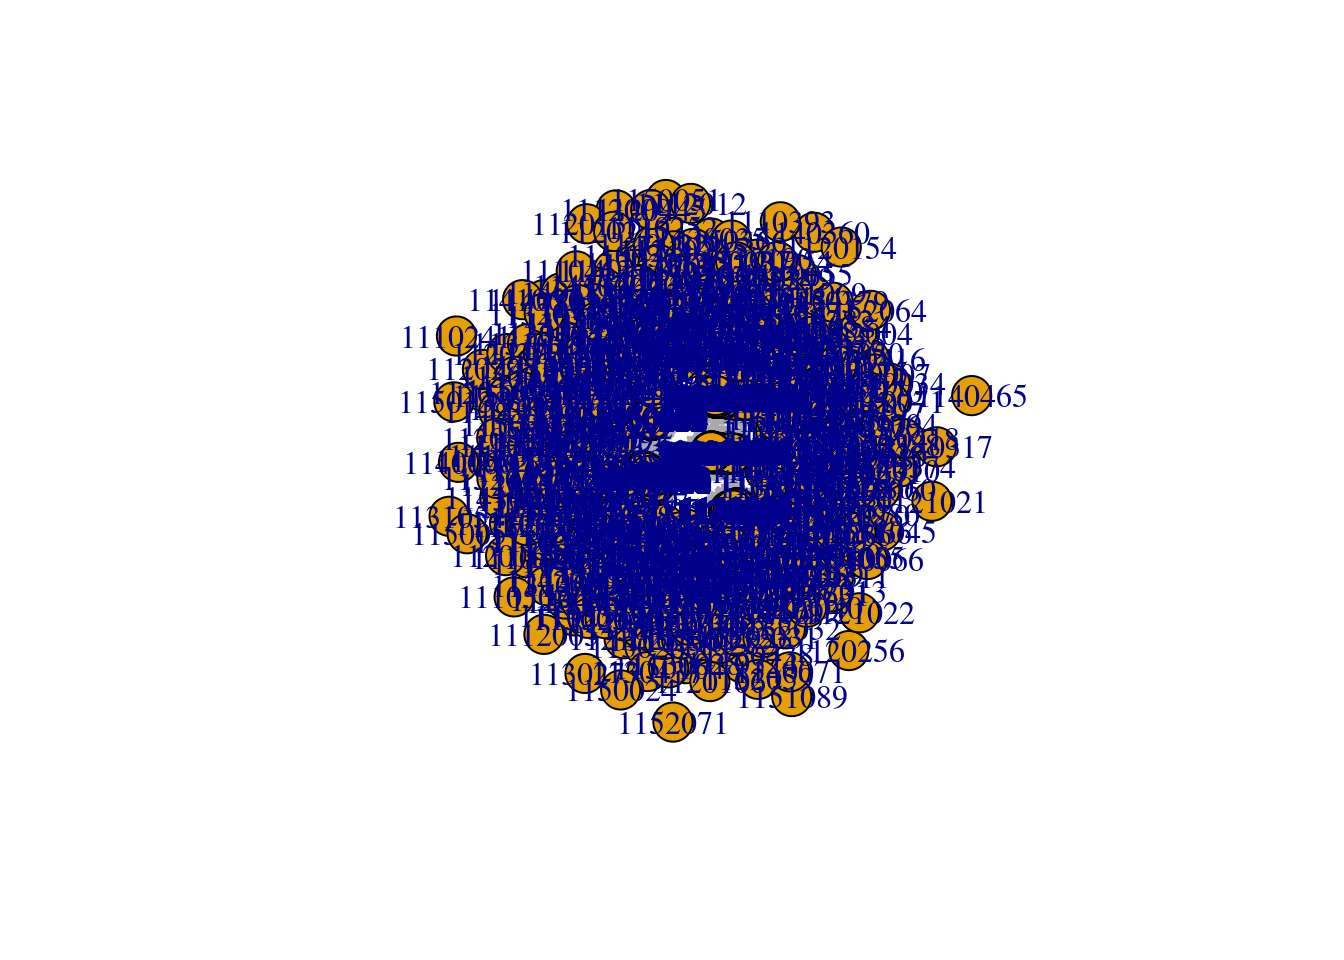
\includegraphics{appliedsnar_files/figure-latex/03-plot-raw-1} 

}

\caption{A not very nice network plot. This is what we get with the default parameters in igraph.}\label{fig:03-plot-raw}
\end{figure}

Not very nice, right? A couple of things with this plot:

\begin{enumerate}
\def\labelenumi{\arabic{enumi}.}
\item
  We are looking at all schools simultaneously, which does not make
  sense. So, instead of plotting \texttt{ig\_year1}, we will focus on
  \texttt{ig\_year1\_111}.
\item
  All the vertices have the same size, and more over, are overalaping.
  So, instead of using the default size, we will size the vertices by
  indegree using the \texttt{degree} function, and passing the vector of
  degrees to \texttt{vertex.size}.\footnote{Figuring out what is the
    optimal vertex size is a bit tricky. Without getting too technical,
    there's no other way of getting \emph{nice} vertex size other than
    just playing with different values of it. A nice solution to this is
    using
    \href{https://www.rdocumentation.org/packages/netdiffuseR/versions/1.17.0/topics/rescale_vertex_igraph}{\texttt{netdiffuseR::igraph\_vertex\_rescale}}
    which rescales the vertices so that these keep their aspect ratio to
    a predefined proportion of the screen.}
\item
  Given the number of vertices in these networks, the labels are not
  useful here. So we will remove them by setting
  \texttt{vertex.label\ =\ NA}. Moreover, we will reduce the size of the
  arrows' tip by setting \texttt{edge.arrow.size\ =\ 0.25}.
\item
  And finally, we will set the color of each vertex to be a function of
  whether the individual is hispanic or not. For this last bit we need
  to go a bit more of programming:
\end{enumerate}

\begin{Shaded}
\begin{Highlighting}[]
\NormalTok{col_hispanic <-}\StringTok{ }\KeywordTok{V}\NormalTok{(ig_year1_}\DecValTok{111}\NormalTok{)}\OperatorTok{$}\NormalTok{hispanic }\OperatorTok{+}\StringTok{ }\DecValTok{1}
\NormalTok{col_hispanic <-}\StringTok{ }\KeywordTok{coalesce}\NormalTok{(col_hispanic, }\DecValTok{3}\NormalTok{) }
\NormalTok{col_hispanic <-}\StringTok{ }\KeywordTok{c}\NormalTok{(}\StringTok{"steelblue"}\NormalTok{, }\StringTok{"tomato"}\NormalTok{, }\StringTok{"white"}\NormalTok{)[col_hispanic]}
\end{Highlighting}
\end{Shaded}

Line by line, we did the following:

\begin{enumerate}
\def\labelenumi{\arabic{enumi}.}
\item
  The first line added one to all no \texttt{NA} values, so that the 0s
  (non-hispanic) turned to 1s and the 1s (hispanic) turned to 2s.
\item
  The second line replaced all \texttt{NA}s with the number 3, so that
  our vector \texttt{col\_hispanic} now ranges from 1 to 3 with no
  \texttt{NA}s in it.
\item
  In the last line we created a vector of colors. Essentially, what we
  are doing here is telling R to create a vector of length
  \texttt{length(col\_hispanic)} by selecting elements by index from the
  vector \texttt{c("steelblue",\ "tomato",\ "white")}. This way, if, for
  example, the first element of the vector \texttt{col\_hispanic} was a
  3, our new vector of colors would have a \texttt{"white"} in it.
\end{enumerate}

To make sure we know we are right, let's print the first 10 elements of
our new vector of colors together with the original \texttt{hispanic}
column:

\begin{Shaded}
\begin{Highlighting}[]
\KeywordTok{cbind}\NormalTok{(}
  \DataTypeTok{original =} \KeywordTok{V}\NormalTok{(ig_year1_}\DecValTok{111}\NormalTok{)}\OperatorTok{$}\NormalTok{hispanic[}\DecValTok{1}\OperatorTok{:}\DecValTok{10}\NormalTok{],}
  \DataTypeTok{colors   =}\NormalTok{ col_hispanic[}\DecValTok{1}\OperatorTok{:}\DecValTok{10}\NormalTok{]}
\NormalTok{  )}
\end{Highlighting}
\end{Shaded}

\begin{verbatim}
##       original colors     
##  [1,] "1"      "tomato"   
##  [2,] "1"      "tomato"   
##  [3,] "0"      "steelblue"
##  [4,] "1"      "tomato"   
##  [5,] "1"      "tomato"   
##  [6,] "1"      "tomato"   
##  [7,] "1"      "tomato"   
##  [8,] "1"      "tomato"   
##  [9,] "0"      "steelblue"
## [10,] "1"      "tomato"
\end{verbatim}

With our nice vector of colors, now we can pass it to
\texttt{plot.igraph} (which we call implicitly by just calling
\texttt{plot}), via the \texttt{vertex.color} argument:

\begin{Shaded}
\begin{Highlighting}[]
\CommentTok{# Fancy graph}
\KeywordTok{set.seed}\NormalTok{(}\DecValTok{1}\NormalTok{)}
\KeywordTok{plot}\NormalTok{(}
\NormalTok{  ig_year1_}\DecValTok{111}\NormalTok{,}
  \DataTypeTok{vertex.size     =} \KeywordTok{degree}\NormalTok{(ig_year1_}\DecValTok{111}\NormalTok{)}\OperatorTok{/}\DecValTok{10} \OperatorTok{+}\DecValTok{1}\NormalTok{,}
  \DataTypeTok{vertex.label    =} \OtherTok{NA}\NormalTok{,}
  \DataTypeTok{edge.arrow.size =}\NormalTok{ .}\DecValTok{25}\NormalTok{,}
  \DataTypeTok{vertex.color    =}\NormalTok{ col_hispanic}
\NormalTok{  )}
\end{Highlighting}
\end{Shaded}

\begin{figure}
\centering
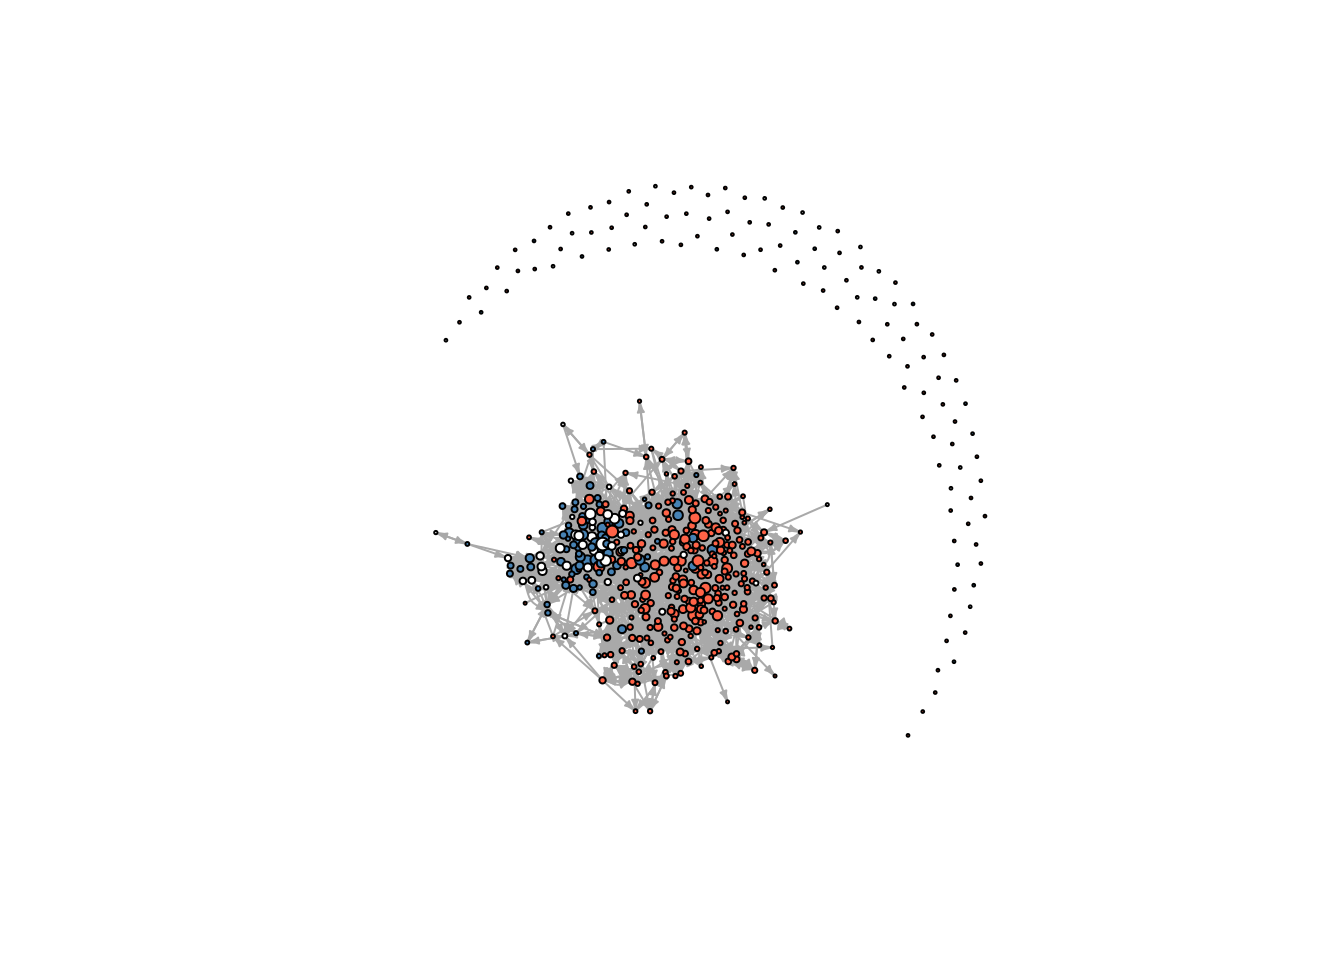
\includegraphics{appliedsnar_files/figure-latex/03-plot-neat1-1.pdf}
\caption{\label{fig:03-plot-neat1}Friends network in time 1 for school 111.}
\end{figure}

Nice! So it does look better. The only problem is that we have a lot of
isolates. Let's try again by drawing the same plot without isolates. To
do so we need to filter the graph, for which we will use the function
\texttt{induced\_subgraph}

\begin{Shaded}
\begin{Highlighting}[]
\CommentTok{# Which vertices are not isolates?}
\NormalTok{which_ids <-}\StringTok{ }\KeywordTok{which}\NormalTok{(}\KeywordTok{degree}\NormalTok{(ig_year1_}\DecValTok{111}\NormalTok{, }\DataTypeTok{mode =} \StringTok{"total"}\NormalTok{) }\OperatorTok{>}\StringTok{ }\DecValTok{0}\NormalTok{)}

\CommentTok{# Getting the subgraph}
\NormalTok{ig_year1_111_sub <-}\StringTok{ }\KeywordTok{induced_subgraph}\NormalTok{(ig_year1_}\DecValTok{111}\NormalTok{, which_ids)}

\CommentTok{# We need to get the same subset in col_hispanic}
\NormalTok{col_hispanic <-}\StringTok{ }\NormalTok{col_hispanic[which_ids]}
\end{Highlighting}
\end{Shaded}

\begin{Shaded}
\begin{Highlighting}[]
\CommentTok{# Fancy graph}
\KeywordTok{set.seed}\NormalTok{(}\DecValTok{1}\NormalTok{)}
\KeywordTok{plot}\NormalTok{(}
\NormalTok{  ig_year1_111_sub,}
  \DataTypeTok{vertex.size     =} \KeywordTok{degree}\NormalTok{(ig_year1_111_sub)}\OperatorTok{/}\DecValTok{5} \OperatorTok{+}\DecValTok{1}\NormalTok{,}
  \DataTypeTok{vertex.label    =} \OtherTok{NA}\NormalTok{,}
  \DataTypeTok{edge.arrow.size =}\NormalTok{ .}\DecValTok{25}\NormalTok{,}
  \DataTypeTok{vertex.color    =}\NormalTok{ col_hispanic}
\NormalTok{  )}
\end{Highlighting}
\end{Shaded}

\begin{figure}
\centering
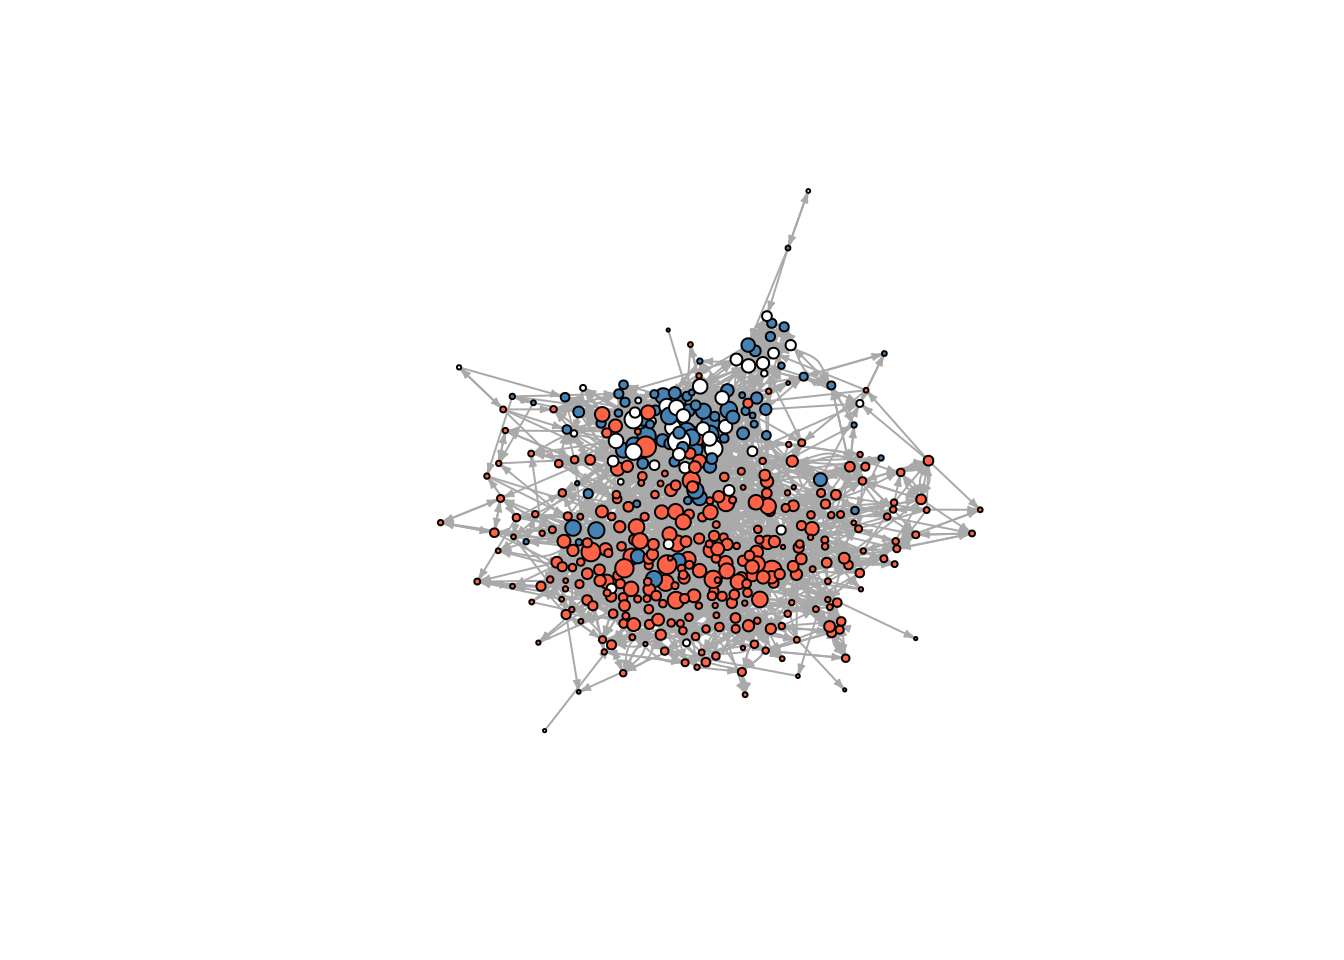
\includegraphics{appliedsnar_files/figure-latex/03-plot-neat2-1.pdf}
\caption{\label{fig:03-plot-neat2}Friends network in time 1 for school 111.
The graph excludes isolates.}
\end{figure}

Now that's better! An interesting pattern that shows up is that
individuals seem to cluster by whether they are hispanic or not.

We can actually write this as a function so that, instead of us copying
and pasting the code \(n\) times (supposing that we want to crate a plot
similar to this \(n\) times). The next subsection does that.

\subsection{Multiple plots}\label{multiple-plots}

\begin{Shaded}
\begin{Highlighting}[]
\NormalTok{myplot <-}\StringTok{ }\ControlFlowTok{function}\NormalTok{(}
\NormalTok{  net,}
\NormalTok{  schoolid,}
  \DataTypeTok{mindgr =} \DecValTok{1}\NormalTok{,}
  \DataTypeTok{vcol   =} \StringTok{"tomato"}\NormalTok{,}
\NormalTok{  ...) \{}
  
  \CommentTok{# Creating a subgraph}
\NormalTok{  subnet <-}\StringTok{ }\KeywordTok{induced_subgraph}\NormalTok{(}
\NormalTok{    net,}
    \KeywordTok{which}\NormalTok{(}\KeywordTok{degree}\NormalTok{(net, }\DataTypeTok{mode =} \StringTok{"all"}\NormalTok{) }\OperatorTok{>=}\StringTok{ }\NormalTok{mindgr }\OperatorTok{&}\StringTok{ }\KeywordTok{V}\NormalTok{(net)}\OperatorTok{$}\NormalTok{school }\OperatorTok{==}\StringTok{ }\NormalTok{schoolid)}
\NormalTok{  )}
  
  \CommentTok{# Fancy graph}
  \KeywordTok{set.seed}\NormalTok{(}\DecValTok{1}\NormalTok{)}
  \KeywordTok{plot}\NormalTok{(}
\NormalTok{    subnet,}
    \DataTypeTok{vertex.size     =} \KeywordTok{degree}\NormalTok{(subnet)}\OperatorTok{/}\DecValTok{5}\NormalTok{,}
    \DataTypeTok{vertex.label    =} \OtherTok{NA}\NormalTok{,}
    \DataTypeTok{edge.arrow.size =}\NormalTok{ .}\DecValTok{25}\NormalTok{,}
    \DataTypeTok{vertex.color    =}\NormalTok{ vcol,}
\NormalTok{    ...}
\NormalTok{    )}
\NormalTok{\}}
\end{Highlighting}
\end{Shaded}

\begin{Shaded}
\begin{Highlighting}[]
\CommentTok{# Plotting all together}
\NormalTok{oldpar <-}\StringTok{ }\KeywordTok{par}\NormalTok{(}\DataTypeTok{no.readonly =} \OtherTok{TRUE}\NormalTok{)}
\KeywordTok{par}\NormalTok{(}\DataTypeTok{mfrow =} \KeywordTok{c}\NormalTok{(}\DecValTok{2}\NormalTok{, }\DecValTok{3}\NormalTok{), }\DataTypeTok{mai =} \KeywordTok{rep}\NormalTok{(}\DecValTok{0}\NormalTok{, }\DecValTok{4}\NormalTok{), }\DataTypeTok{oma=} \KeywordTok{c}\NormalTok{(}\DecValTok{1}\NormalTok{, }\DecValTok{0}\NormalTok{, }\DecValTok{0}\NormalTok{, }\DecValTok{0}\NormalTok{))}
\KeywordTok{myplot}\NormalTok{(ig_year1, }\DecValTok{111}\NormalTok{, }\DataTypeTok{vcol =} \StringTok{"tomato"}\NormalTok{)}
\KeywordTok{myplot}\NormalTok{(ig_year1, }\DecValTok{112}\NormalTok{, }\DataTypeTok{vcol =} \StringTok{"steelblue"}\NormalTok{)}
\KeywordTok{myplot}\NormalTok{(ig_year1, }\DecValTok{113}\NormalTok{, }\DataTypeTok{vcol =} \StringTok{"black"}\NormalTok{)}
\KeywordTok{myplot}\NormalTok{(ig_year1, }\DecValTok{114}\NormalTok{, }\DataTypeTok{vcol =} \StringTok{"gold"}\NormalTok{)}
\KeywordTok{myplot}\NormalTok{(ig_year1, }\DecValTok{115}\NormalTok{, }\DataTypeTok{vcol =} \StringTok{"white"}\NormalTok{)}
\KeywordTok{par}\NormalTok{(oldpar)}

\CommentTok{# A fancy legend}
\KeywordTok{legend}\NormalTok{(}
  \StringTok{"bottomright"}\NormalTok{,}
  \DataTypeTok{legend =} \KeywordTok{c}\NormalTok{(}\DecValTok{111}\NormalTok{, }\DecValTok{112}\NormalTok{, }\DecValTok{113}\NormalTok{, }\DecValTok{114}\NormalTok{, }\DecValTok{115}\NormalTok{),}
  \DataTypeTok{pt.bg  =} \KeywordTok{c}\NormalTok{(}\StringTok{"tomato"}\NormalTok{, }\StringTok{"steelblue"}\NormalTok{, }\StringTok{"black"}\NormalTok{, }\StringTok{"gold"}\NormalTok{, }\StringTok{"white"}\NormalTok{),}
  \DataTypeTok{pch    =} \DecValTok{21}\NormalTok{,}
  \DataTypeTok{cex    =} \DecValTok{1}\NormalTok{,}
  \DataTypeTok{bty    =} \StringTok{"n"}\NormalTok{,}
  \DataTypeTok{title  =} \StringTok{"School"}
\NormalTok{  )}
\end{Highlighting}
\end{Shaded}

\begin{figure}
\centering
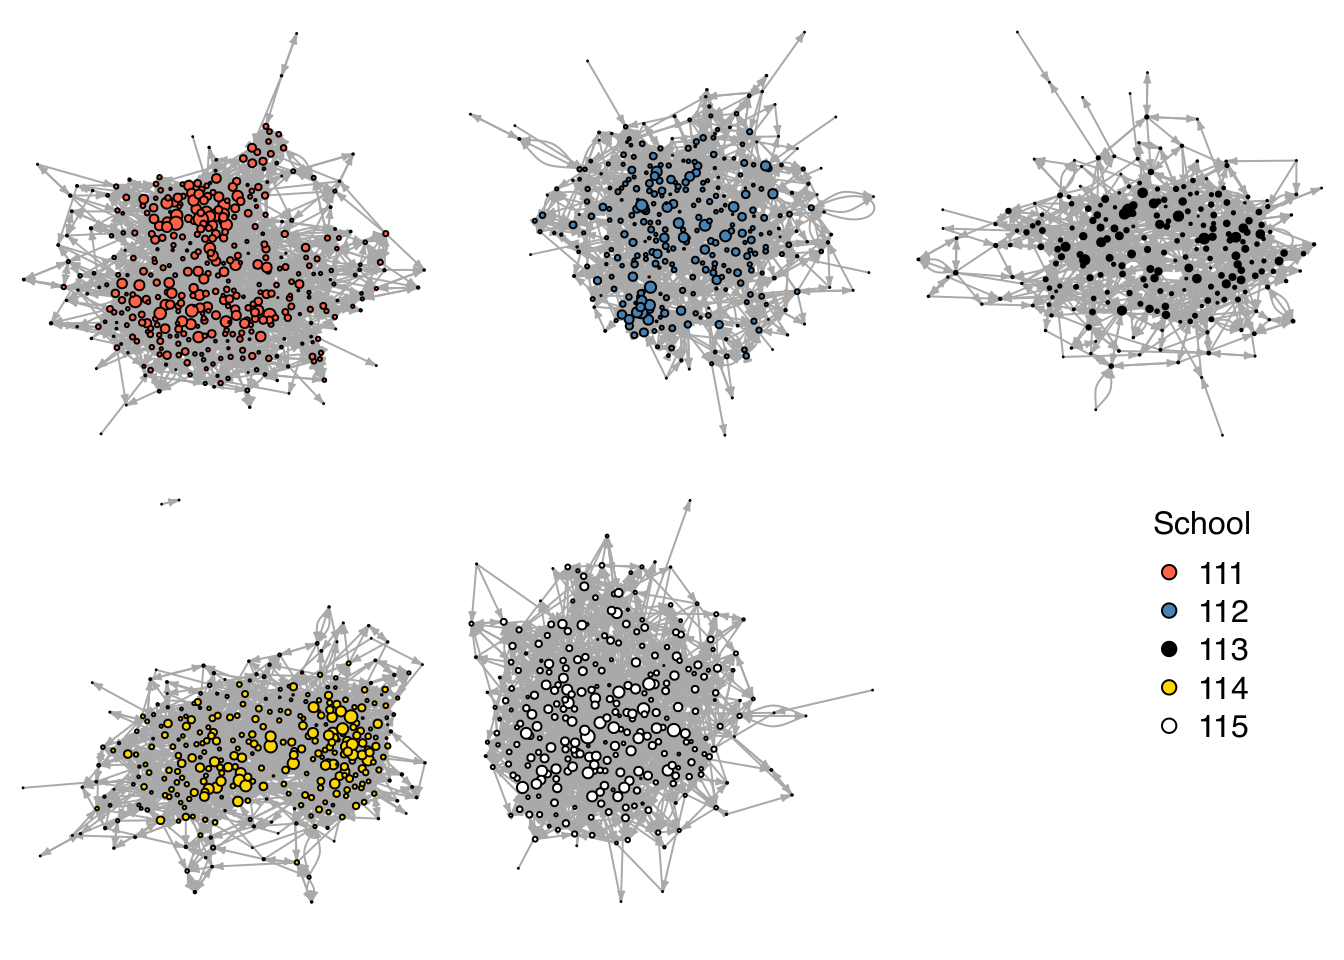
\includegraphics{appliedsnar_files/figure-latex/03-myplot-call-1.pdf}
\caption{\label{fig:03-myplot-call}All 5 schools in time 1. Again, the
graphs exclude isolates.}
\end{figure}

\begin{itemize}
\item
  \texttt{oldpar\ \textless{}-\ par(no.readonly\ =\ TRUE)} This line
  stores the current parameters for plotting. Since we are going to be
  changing them, we better make sure we are able to go back!.
\item
  \texttt{par(mfrow\ =\ c(2,\ 3),\ mai\ =\ rep(0,\ 4),\ oma=rep(0,\ 4))}
  Here we are setting various things at the same time. \texttt{mfrow}
  specifies how many \emph{figures} will be drawn and in what order, in
  particular, we are asking the plotting device to allow for 2*3 = 6
  plots organized in 2 rows and 3 columns, and these will be drawn by
  row.

  \texttt{mai} specifies the size of the margins in inches. Setting all
  margins equal to zero (which is what we are doing now) gives more
  space to the network itself. The same is true for \texttt{oma}. See
  \texttt{?par} for more info.
\item
  \texttt{myplot(ig\_year1,\ ...)} This is simply calling our plotting
  function. The neat part of this is that, since we set
  \texttt{mfrow\ =\ c(2,\ 3)}, R takes care of \emph{distributing} the
  plots in the device.
\item
  \texttt{par(oldpar)} Finally, this line allows us to restore the
  plotting parameters.
\end{itemize}

\chapter{Applications}\label{applications}

Some \emph{significant} applications are demonstrated in this chapter.

\section{Example one}\label{example-one}

\section{Example two}\label{example-two}

\chapter{Final Words}\label{final-words}

We have finished a nice book.

\cleardoublepage 

\appendix


\chapter{Datasets}\label{datasets}

\hypertarget{sns-data}{\section{SNS data}\label{sns-data}}

\subsection{About the data}\label{about-the-data}

\begin{itemize}
\item
  This data is part of the NIH Challenge grant \# RC 1RC1AA019239
  ``Social Networks and Networking That Puts Adolescents at High Risk''.
\item
  In general terms, the SNS's goal was(is) ``Understand the network
  effects on risk behaviors such as smoking initiation and substance
  use''.
\end{itemize}

\subsection{Variables}\label{variables}

The data has a \emph{wide} structure, which means that there is one row
per individual, and that dynamic attributes are represented as one
column per time.

\begin{itemize}
\item
  \texttt{photoid} Photo id at the school level (can be repeated across
  schools).
\item
  \texttt{school} School id.
\item
  \texttt{hispanic} Indicator variable that equals 1 if the indivual
  ever reported himself as hispanic.
\item
  \texttt{female1}, \ldots{}, \texttt{female4} Indicator variable that
  equals 1 if the individual reported to be female at the particular
  wave.
\item
  \texttt{grades1},\ldots{}, \texttt{grades4} Academic grades by wave.
  Values from 1 to 5, with 5 been the best.
\item
  \texttt{eversmk1}, \ldots{}, \texttt{eversmk4} Indicator variable of
  ever smoking by wave. A one indicated that the individual had smoked
  at the time of the survey.
\item
  \texttt{everdrk1}, \ldots{}, \texttt{everdrk4} Indicator variable of
  ever drinking by wave. A one indicated that the individual had drink
  at the time of the survey.
\item
  \texttt{home1}, \ldots{}, \texttt{home4} Factor variable for home
  status by wave. A one indicates home ownership, a 2 rent, and a 3 a
  ``I don't know''.
\end{itemize}

During the survey, participants were asked to name up to 19 of their
school friends:

\begin{itemize}
\item
  \texttt{sch\_friend11}, \ldots{}, \texttt{sch\_friend119} School
  friends nominations (19 in total) for wave 1. The codes are mapped to
  the variable \texttt{photoid}.
\item
  \texttt{sch\_friend21}, \ldots{}, \texttt{sch\_friend219} School
  friends nominations (19 in total) for wave 2. The codes are mapped to
  the variable \texttt{photoid}.
\item
  \texttt{sch\_friend31}, \ldots{}, \texttt{sch\_friend319} School
  friends nominations (19 in total) for wave 3. The codes are mapped to
  the variable \texttt{photoid}.
\item
  \texttt{sch\_friend41}, \ldots{}, \texttt{sch\_friend419} School
  friends nominations (19 in total) for wave 4. The codes are mapped to
  the variable \texttt{photoid}.
\end{itemize}

\bibliography{book.bib,packages.bib}


\end{document}
